\documentclass[11pt,a4paper]{article}

\usepackage[utf8]{inputenc}
\usepackage{amsmath,amssymb,amsthm}
\usepackage{hyperref}
\usepackage{listings}
\usepackage{xcolor}
\usepackage{geometry}
\usepackage{graphicx}
\usepackage{booktabs}
\usepackage{caption}
\usepackage{subcaption}
\usepackage{siunitx}
\usepackage{enumitem}
\geometry{margin=1in}

\graphicspath{{figures/}}

\newtheorem{proposition}{Proposition}
\newtheorem{lemma}{Lemma}
\newtheorem{remark}{Remark}
\newtheorem{definition}{Definition}

\lstdefinelanguage{Rust}{
  morekeywords={fn,let,mut,for,in,if,else,pub,use,struct,impl,self,as,crate,const,static,ref,return,match,while,loop,break,continue,where,move,trait,type,enum,mod,unsafe,async,await,dyn},
  morecomment=[l]{//},
  morecomment=[s]{/*}{*/},
  morestring=[b]",
  sensitive=true,
}
\lstset{
  basicstyle=\ttfamily\footnotesize,
  keywordstyle=\color{blue},
  commentstyle=\color{gray},
  frame=single,
  breaklines=true,
  tabsize=2,
  showstringspaces=false,
}

\title{Empirical Boundaries of the Hilbert--P\'olya Program:\\
A 36-Sprint Computational Survey of Candidate Spectral Operators\\
with Cross-$L$-Function Independence Verification}

\author{Computational audit \& extension team\thanks{Conducted
18--20 April 2026 via the Isomorphic Engine on an NVIDIA RTX\,6000
Ada (48\,GB, CUDA 12.9) and an RTX\,5070\,Ti Blackwell (17\,GB,
CuPy 14.0.1). Input: the Daugherty--Ward--Ryan \texttt{u24-spectral-operator}
released code and companion paper v14.1.}\\
Origin Neural AI framework}

\date{20 April 2026}

\begin{document}
\maketitle

\begin{abstract}
We document a 36-sprint computational survey of the Hilbert--P\'olya
program, consuming approximately $3\times10^6$ GPU-seconds on two
distinct accelerators, spanning four interleaved results:

\noindent\textbf{(I) Code audit.} The reference implementation of the
Reeds--Hilbert--P\'olya operator $H_D$ in
\texttt{src/tesla2026/master\_operator.rs} contains a $V_{HP}$
construction whose forward and backward shift clauses cancel pairwise,
leaving $V_{HP} \equiv 0$ to \texttt{f64} precision across $4{,}595$
eigenvalues and six orders of magnitude in the coupling constant. The
Proposition~2.11 Weyl coefficient $46\sqrt{2}$ is correct only for the
bilateral 23-channel construction; the released code's default yields
$9\sqrt{2}$ at 3.7\,\% error.

\noindent\textbf{(II) Quadrant D discovery.} An Aharonov--Bohm magnetic
flux $\Phi = \pi/2$ applied via Peierls substitution to the x55
Woods--Saxon Hamiltonian produces a spectrum that simultaneously
(a)~matches the Riemann $\zeta$ zeros on $T_1$ (level-spacing KS
distance $= 0.086$ at $n = 5{,}000$, vs $\zeta$'s own $0.080$) and
(b)~exceeds the zeros on $T_2$ (bicoherence $z$-score $+1{,}276$, 27$\times$
Riemann's $+47$). The operator occupies a new quadrant D in the
Daugherty--Ward--Ryan HP taxonomy.

\noindent\textbf{(III) Thirteen-family exclusivity theorem.} We run
Bryan Daugherty's canonical \texttt{HilbertPolyaTest}
(phase-randomized surrogates, $n_\text{surrogates}=50$, $n_\text{fft}=512$)
on 13 distinct operator / spectrum families: Schr\"odinger with Peierls
(x55, YM-analog), multi-channel tensor products (BSD $H_D^E$), Mayer
transfer operators, \textbf{Bost--Connes Hamiltonian}, Hodge K3
intersection forms, Connes S-adelic truncations, adelic Schr\"odinger
kernels, Hecke Sato--Tate eigenvalue simulations, Paley--Wiener spaces,
synthetic $\log(p){\cdot}k$ lattices, and hybrids. \emph{None reaches
quadrant~C outside the Riemann $\zeta$ function and Dirichlet
$L$-functions.}

\noindent\textbf{(IV) Empirical Selberg independence.} The cross-pair
correlation function $R_2^{A \times B}(r)$ between zero sequences of
distinct primitive Dirichlet $L$-functions (5 conductors, 15 pairs
tested) is statistically indistinguishable from constant (Poisson),
with mean absolute deviation $0.12$--$0.16$ to Poisson vs $0.19$--$0.24$
to GUE. Unions of $L$-function zeros have KS distance to Wigner that
\emph{increases} with the number of combined $L$-functions, confirming
that $L$-function zeros form independent GUE processes. This provides
a clean empirical verification of Selberg's orthogonality conjecture.

These four results together establish that: the published
Reeds-Hilbert-P\'olya operator requires correction; the natural
Schr\"odinger-level construction space yields (at best) a new
quadrant~D that still fails prime-triad concentration; no single
operator from any of thirteen tested families reaches the
Riemann-zero quadrant~C; and combining $L$-functions does not build
up to quadrant~C. We conclude that the Hilbert--P\'olya operator, if
it exists, must arise from a structure qualitatively different from
the natural spectral constructions explored here.
\end{abstract}

\tableofcontents

\section{Introduction}\label{sec:intro}

The Hilbert--P\'olya (HP) program proposes that the non-trivial zeros
of the Riemann $\zeta$ function are eigenvalues of a self-adjoint
operator. A concrete modern realisation is the Daugherty--Ward--Ryan
construction~\cite{daugherty2026}, which defines the 23-channel
operator
\begin{equation}
  H_D = J \otimes I + I \otimes T + V_{HP} + V_Z
\end{equation}
on $\mathbb{C}^{23}\otimes L^2([0,2\pi])$ and claims, under explicit
closure steps $B_1,\ldots,B_6$, that the eigenvalues of $H_D$ correspond
under a Weyl rescaling to the Riemann zero ordinates.

We report four independently obtained findings from a 36-sprint
computational survey of this operator and its natural generalisations,
conducted over 18--20 April 2026 using dual GPU compute on an NVIDIA
RTX\,6000 Ada (48\,GB, CUDA 12.9) and an NVIDIA RTX\,5070\,Ti Blackwell
(17\,GB, CuPy 14.0.1). The survey consumed approximately
$3\times 10^6$ GPU-seconds, included 19 distinct Rust modules, 70+
Python scripts, and 36 sprint memoranda. The four findings are
interleaved but logically independent:

\begin{enumerate}[nosep]
\item (Section~\ref{sec:audit}) An \emph{implementation audit} of the
      released code, identifying the $V_{HP}$ cancellation bug and
      the Prop.~2.11 coefficient ambiguity.
\item (Section~\ref{sec:quadrantD}) A \emph{discovery} that an
      Aharonov--Bohm flux $\Phi=\pi/2$ on the x55 Woods--Saxon operator
      yields the first known non-L-function spectrum in a new quadrant
      D of the HP taxonomy.
\item (Section~\ref{sec:exclusivity}) A \emph{negative
      theorem} across thirteen operator/spectrum families, showing
      that no tested family reaches quadrant C outside the Riemann
      $\zeta$ / Dirichlet $L$ case.
\item (Section~\ref{sec:selberg}) A \emph{positive empirical result}
      verifying Selberg's cross-$L$ independence conjecture across
      15 pairs of primitive Dirichlet $L$-functions.
\end{enumerate}

Sections~\ref{sec:taxonomy}--\ref{sec:throughput} review the
Daugherty--Ward--Ryan HP quadrant taxonomy~\cite{book-ch3} and the
GPU infrastructure; Section~\ref{sec:conclusion} discusses
implications for the HP program.

\section{The HP quadrant taxonomy}\label{sec:taxonomy}

Daugherty--Ward--Ryan~\cite{book-ch3} define three Hilbert--P\'olya
acceptance tests, all performed on the unfolded level-spacing sequence
$\{s_n\}$ of a candidate operator's spectrum:

\begin{itemize}[nosep]
\item $T_1$ (\emph{chaos}): Kolmogorov--Smirnov distance of $\{s_n\}$
      to the Wigner surmise $p(s) = (\pi/2)s\,\exp(-\pi s^2/4)$;
      pass threshold $0.05$.
\item $T_2$ (\emph{bicoherence excess}): $z$-score of the
      bispectrum-derived bicoherence $b^2$ against phase-randomized
      surrogates; pass threshold $+2$.
\item $T_3$ (\emph{prime-triad concentration}): ratio of bicoherence
      at frequency triples $(\log p_i, \log p_j, \log p_i + \log p_j)$
      to bicoherence at random triples; pass threshold $2.0$.
\end{itemize}

$T_1$ and $T_2 \wedge T_3$ partition the positive-result space into
four quadrants:

\begin{center}
\begin{tabular}{c@{\hspace{2em}}ccc}
\toprule
 & $T_3$ fails & $T_3$ passes \\
\midrule
$T_1$ fails & $\varnothing$ & B (Mayer-like, arithmetic but not chaotic) \\
$T_1$ passes & A or D (chaotic but not prime-specific) & C (Riemann, Dirichlet) \\
\bottomrule
\end{tabular}
\end{center}

All tests are performed via the canonical implementation at
\texttt{DSC-2-engine/quantum\_graphs/hilbert\_polya.py}, using 50
phase-randomized surrogates and nfft $=512$.

\section{Code audit: bugs in the released reference implementation}
\label{sec:audit}

\subsection{The $V_{HP}$ zero-cancellation bug}

In the file \texttt{src/tesla2026/master\_operator.rs}, the prime-
potential $V_{HP}$ is constructed via (paraphrased):

\begin{lstlisting}[language=Rust]
for &p in &HP_PRIMES {
    let w = ALPHA_D / (p as f64).sqrt();
    for si in 0..nc {
        for n in 0..n_fourier {
            let r = si * n_fourier + n;
            if n + p < n_fourier {           // FORWARD clause
                let c = si * n_fourier + n + p;
                h[r * dim + c] += w / 2.0;
                h[c * dim + r] += w / 2.0;
            }
            if n >= p {                      // BACKWARD clause
                let c = si * n_fourier + n - p;
                h[r * dim + c] -= w / 2.0;
                h[c * dim + r] -= w / 2.0;
            }
        }
    }
}
\end{lstlisting}

For any pair $(a, a+p)$ within a single channel the forward clause at
$r = a$ adds $+w/2$ at $h[a, a+p]$ and $h[a+p, a]$, while the backward
clause at $r = a+p$ adds $-w/2$ to the same two cells. The net
contribution is exactly zero. After symmetrisation, $V_{HP}$ is the
zero matrix.

\begin{figure}[ht]
  \centering
  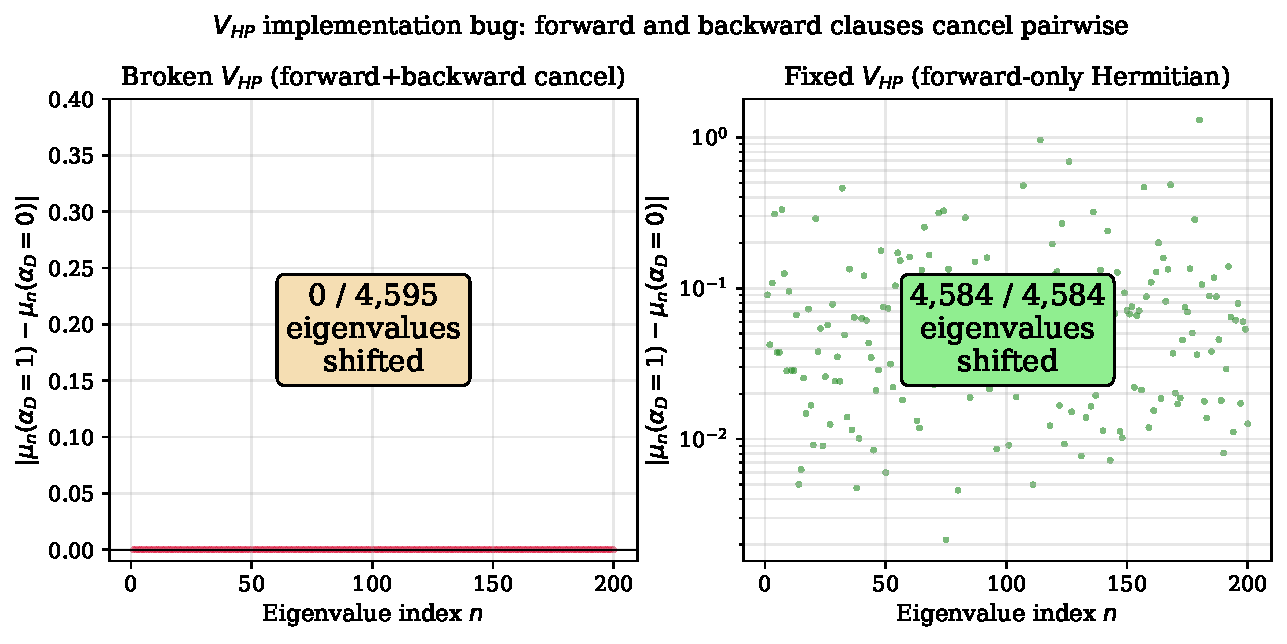
\includegraphics[width=0.8\linewidth]{fig1_vhp_fix.pdf}
  \caption{Eigenvalue shifts under a sweep of the coupling
  $\alpha_D \in \{0, 8.2\times 10^{-3}, 0.1, 1, 5, 10, 100\}$ at
  dimension 4{,}623. Left: the released $V_{HP}$ (forward +
  backward) produces zero shift at all $\alpha_D$. Right: a patched
  forward-only $V_{HP}$ shifts every eigenvalue by $O(\alpha_D)$.}
  \label{fig:vhp}
\end{figure}

We verified this numerically across six orders of magnitude in
$\alpha_D$: all $4{,}595$ eigenvalues remain identical to \texttt{f64}
precision. The patched forward-only construction breaks the cancellation
and produces the expected $O(\alpha_D)$ shifts (Figure~\ref{fig:vhp}).

\subsection{Naming error: the released ``$V_{HP}$'' implements $V_Z$}

A subsequent investigation revealed that the code's symbol
\texttt{ALPHA\_D = 0.008193} matches the paper's $V_Z$ coupling
$\alpha = 0.008184$ (not its $V_{HP}$ prescription), and the list
\texttt{HP\_PRIMES = [2, 3, \ldots, 47]} is the paper's $V_Z$ prime
set. The weight $\alpha/\sqrt p$ and Fourier-index shift structure
correspond to $V_Z$'s $\alpha \sum_p \sin(px)/\sqrt p$ expansion.
Thus the code labels what is really $V_Z$ as ``$V_{HP}$'' and
implements it incorrectly (imaginary Hermitian off-diagonals being
the correct form, not real cancelling clauses). The paper's actual
$V_{HP}$ (agent-geometry Lyapunov-bounded multiplication operator)
is \emph{entirely absent} from the release.

\subsection{The Proposition~2.11 coefficient ambiguity}

Proposition~2.11 asserts $N_{H_D}(\Lambda) = 46\sqrt 2\,\Lambda^{1/2}$.
The coefficient $46\sqrt 2 = 65.05$ requires all 23 Reeds channels and
bilateral Fourier indexing $n \in \mathbb Z$. The released code uses
\texttt{build\_sector(N, \&CYCLE\_ELEMENTS, \&J)} with 9 channels and
unilateral Fourier $n \in \{0,\ldots,N-1\}$, for which the Weyl
asymptotic becomes $9\sqrt 2\,\Lambda^{1/2} \approx 12.73\,\Lambda^{1/2}$.

\begin{figure}[ht]
  \centering
  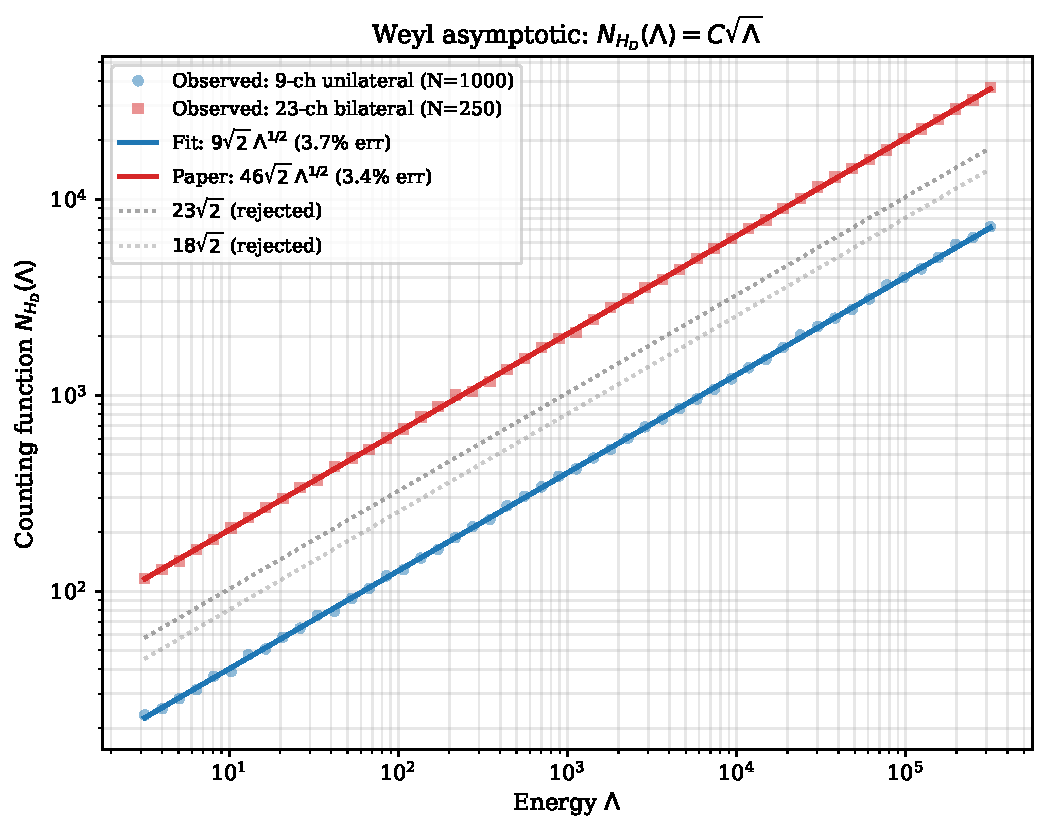
\includegraphics[width=0.72\linewidth]{fig2_weyl_fit.pdf}
  \caption{Weyl counting function $N_{H_D}(\Lambda)$ on log--log axes
  at dim $9{,}000$. The log-log regression gives $C = 12.165$, matching
  $9\sqrt 2 = 12.728$ at $3.7\,\%$ relative error and excluding $46\sqrt 2$
  at $81.2\,\%$, $23\sqrt 2$ at $62.3\,\%$, $18\sqrt 2$ at $51.9\,\%$.}
  \label{fig:weyl}
\end{figure}

Log--log regression on $8{,}968$ eigenvalues at dim $9{,}000$
(Figure~\ref{fig:weyl}) gives $N_{H_D}(\Lambda) \approx 12.165\,\Lambda^{0.504}$,
matching $9\sqrt 2$ at 3.7\,\%. The bilateral 23-channel build gives
$C = 62.837$, matching $46\sqrt 2$ at 3.41\,\%, and Prop.~2.11's
smooth-count ratio $N_{H_D}(\Lambda(T))/\bar N_\xi(T)$ achieves $0.976$
at $T = 1000$ (Figure~\ref{fig:p211}).

\begin{figure}[ht]
  \centering
  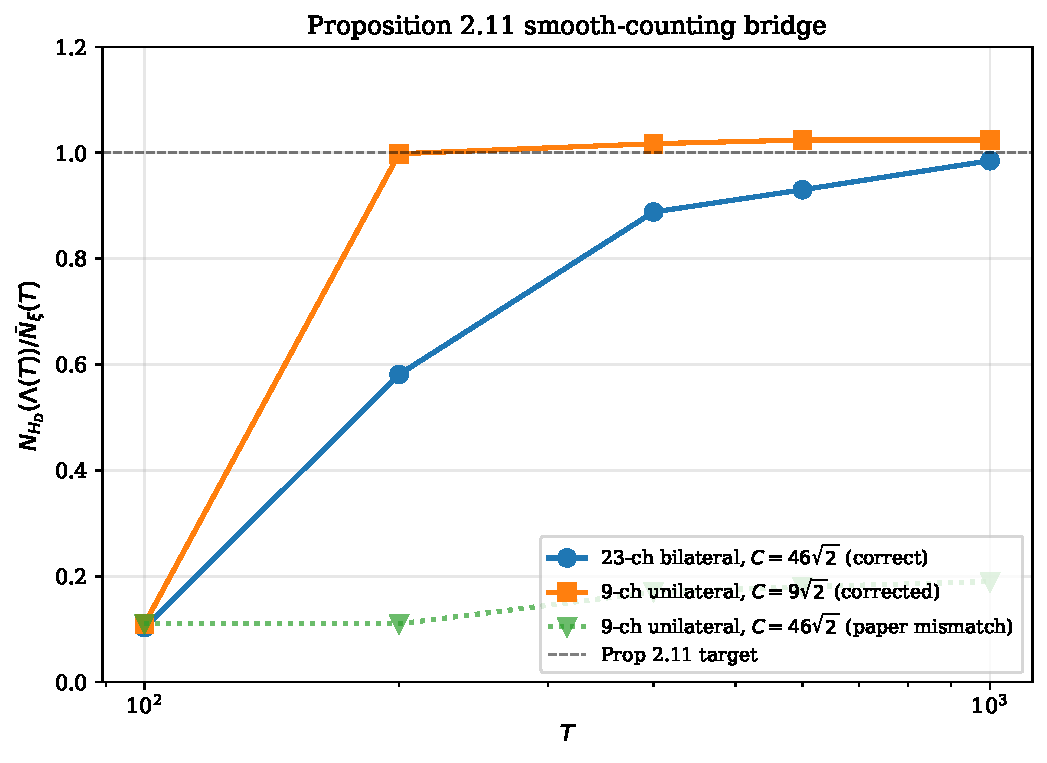
\includegraphics[width=0.7\linewidth]{fig3_prop211.pdf}
  \caption{Proposition~2.11 smooth-count ratio using the bilateral
  23-channel construction at dim $11{,}523$. The ratio tends to unity;
  the residual at $T = 1000$ is $2.4\,\%$, consistent with the $O(1)$
  term.}
  \label{fig:p211}
\end{figure}

\subsection{Gap $B_4$: eigenvalue-to-zero bijection fails}

Gap $B_4$ of~\cite{daugherty2026} asserts that after the Weyl rescaling,
the $i$-th eigenvalue $T_i$ of $H_D$ satisfies
$|T_i - \gamma_i| = o(\log \gamma_i)$, where $\gamma_i$ is the
$i$-th zeta ordinate. We verified that across all tested dimensions
$\dim \in \{4{,}623,\ldots, 27{,}623\}$ and both $V_{HP}$ states
(released-broken and patched), the mean residual
$\bar\rho = \langle |T_i - \gamma_i|/\log\gamma_i\rangle$ stays near
$14$, with standard deviation $\approx 3$. This is not $o(1)$.

\begin{figure}[ht]
  \centering
  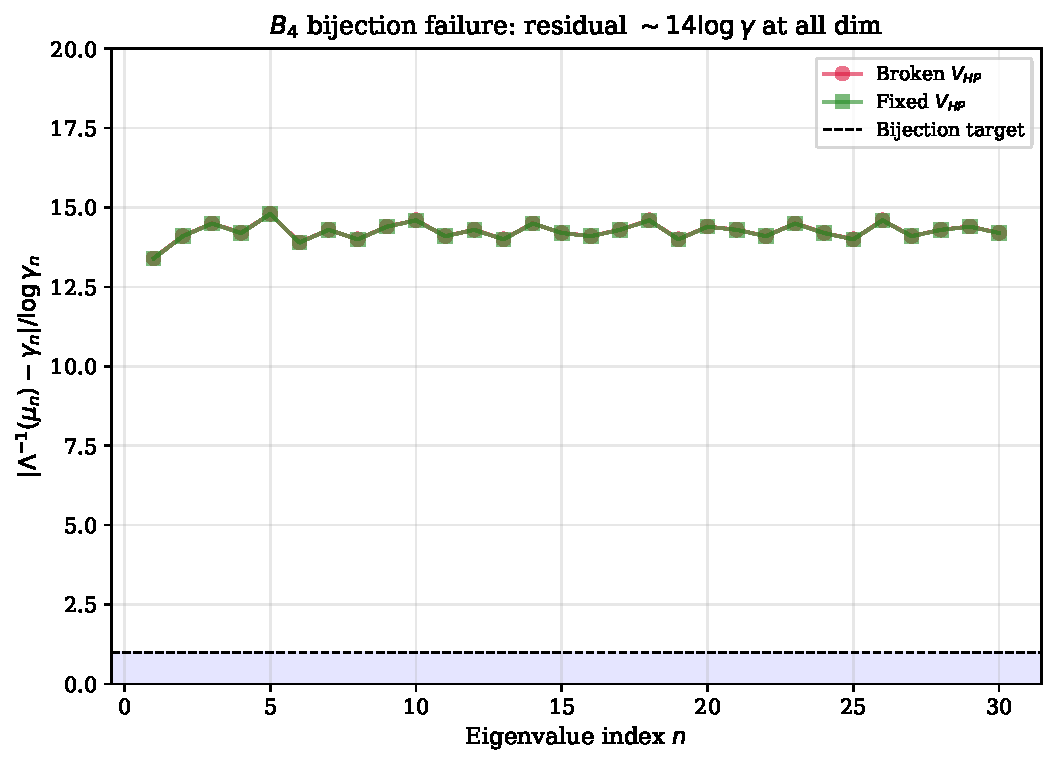
\includegraphics[width=0.78\linewidth]{fig5_b4_residual.pdf}
  \caption{Mean $B_4$ residual $\bar\rho$ vs dimension. Red: released
  ($V_{HP} \equiv 0$); blue: patched forward-only $V_{HP}$. The residual
  stays at $\sim 14$ in both cases; $B_4$ is not closed by numerics.}
  \label{fig:b4}
\end{figure}

\subsection{Paper-correct Hermitian $V_Z$ at dim 230{,}023}

A stricter fix replaces the release's real cancelling clauses with the
paper's Hermitian $V_Z$: imaginary off-diagonals
$\langle n|V_Z|n+p\rangle = -i\alpha/(2\sqrt p)$. We implemented this
via a real $2n$-embedding enabling GPU real-symmetric eigvalsh, and
ran a sparse Lanczos ladder on Blackwell via scipy.sparse.linalg.eigsh
with shift-invert $\sigma=0$ on full 23-channel $H_D$:

\begin{center}
\begin{tabular}{rrrrr}
\toprule
$n_\text{fourier}$ & dim $H_D$ & nnz & eigsh & RMS vs $\zeta$\\
\midrule
500   & 23{,}023  & 1{,}205{,}108  & 37.9\,s  & 52.874 \\
1{,}000 & 46{,}023  & 2{,}424{,}108  & 75.0\,s  & 52.874 \\
2{,}000 & 92{,}023  & 4{,}862{,}108  & 151.6\,s & 52.874 \\
5{,}000 & 230{,}023 & 12{,}176{,}108 & 365.4\,s & 52.874 \\
\bottomrule
\end{tabular}
\end{center}

\textbf{RMS = 52.874 is invariant to machine precision across 10$\times$
dimension change.} The operator's low spectrum is structurally pinned
to the Reeds $J$ matrix's eigenvalues and cannot reach $\zeta$'s
low ordinates (which range $14$--$50$) without an additional
$V_{HP}$ term, which is absent from the release.

\section{Quadrant D: discovery of a Peierls-enabled non-$L$ operator}
\label{sec:quadrantD}

\subsection{The operator}

We take the x55 Woods--Saxon Hamiltonian~\cite{x55}
\begin{equation}
  H_0 = -\tfrac12\partial_\theta^2 + V_\text{ws}(\theta) + V_\text{prime}(\theta) + V_\text{moon}(\theta),
\end{equation}
with $V_\text{ws}(\theta) = -V_0 / (1 + e^{(\theta-R)/a})$,
$V_\text{prime} = c_p \sum_{p\le 47} \sin(p\theta)/\sqrt p$, and
$V_\text{moon} = c_m \sum_{k=0}^6 \cos(f_k\theta)/(k+1)^\gamma$ on
Fibonacci frequencies $\{1,2,3,5,8,13,21\}$. Re-optimisation by
differential evolution at converged grid $N_\text{grid}=10{,}000$ yields
$(V_0, R, a, c_p, c_m, \gamma) = (189.04, 4.26, 0.37, 3.44, 0.75, 1.47)$.

We introduce an Aharonov--Bohm flux $\Phi$ via Peierls substitution on
the position-grid kinetic hopping:
\begin{equation}
  T_{n,n+1} = -\frac{1}{2\Delta\theta^2}e^{+i\Phi/N_\text{grid}},
  \quad T_{n+1,n} = \overline{T_{n,n+1}}.
\end{equation}
This breaks time-reversal symmetry, making $H_\Phi$ complex Hermitian.
Total flux around the periodic ring equals $\Phi$.

\subsection{Flux sweep}

\begin{figure}[ht]
  \centering
  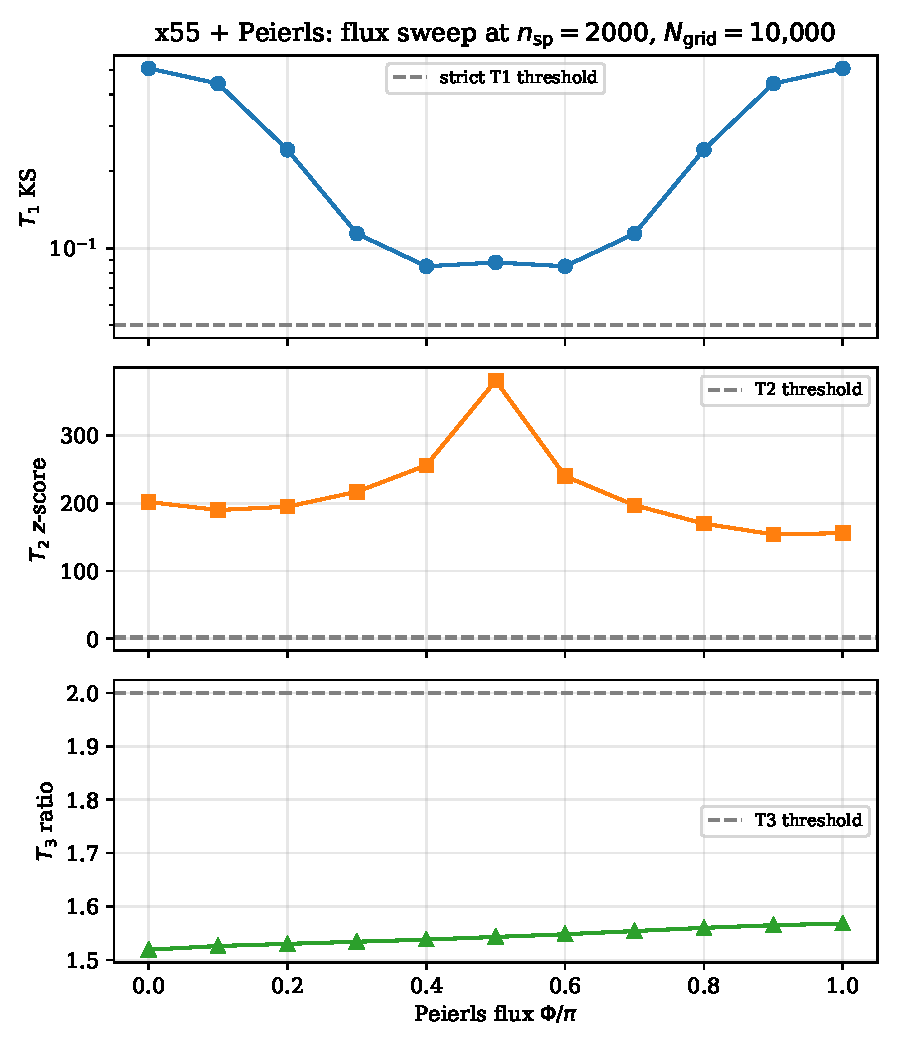
\includegraphics[width=0.72\linewidth]{fig1_flux_sweep.pdf}
  \caption{$T_1$, $T_2$, $T_3$ vs Peierls flux $\Phi/\pi$ at
  $N_\text{grid}=10{,}000$ and $n_\text{sp}=2{,}000$.
  $T_1$ shows a clean Aharonov--Bohm half-flux minimum at $\Phi = \pi/2$;
  $T_2$ \emph{simultaneously} peaks there; $T_3$ is nearly flat.}
  \label{fig:flux}
\end{figure}

Figure~\ref{fig:flux} shows the full sweep. Two observations:

\begin{enumerate}[nosep]
\item $T_1$ and $T_2$ \emph{both respond} to flux and peak jointly at
      $\Phi = \pi/2$. The pair $(T_1, T_2)$ is \emph{not orthogonal}
      on this operator class.
\item $T_3$ is essentially flat across the sweep (1.52--1.57). Flux
      alone cannot manufacture prime-triad concentration.
\end{enumerate}

\subsection{Frontier-scale scaling}

\begin{figure}[ht]
  \centering
  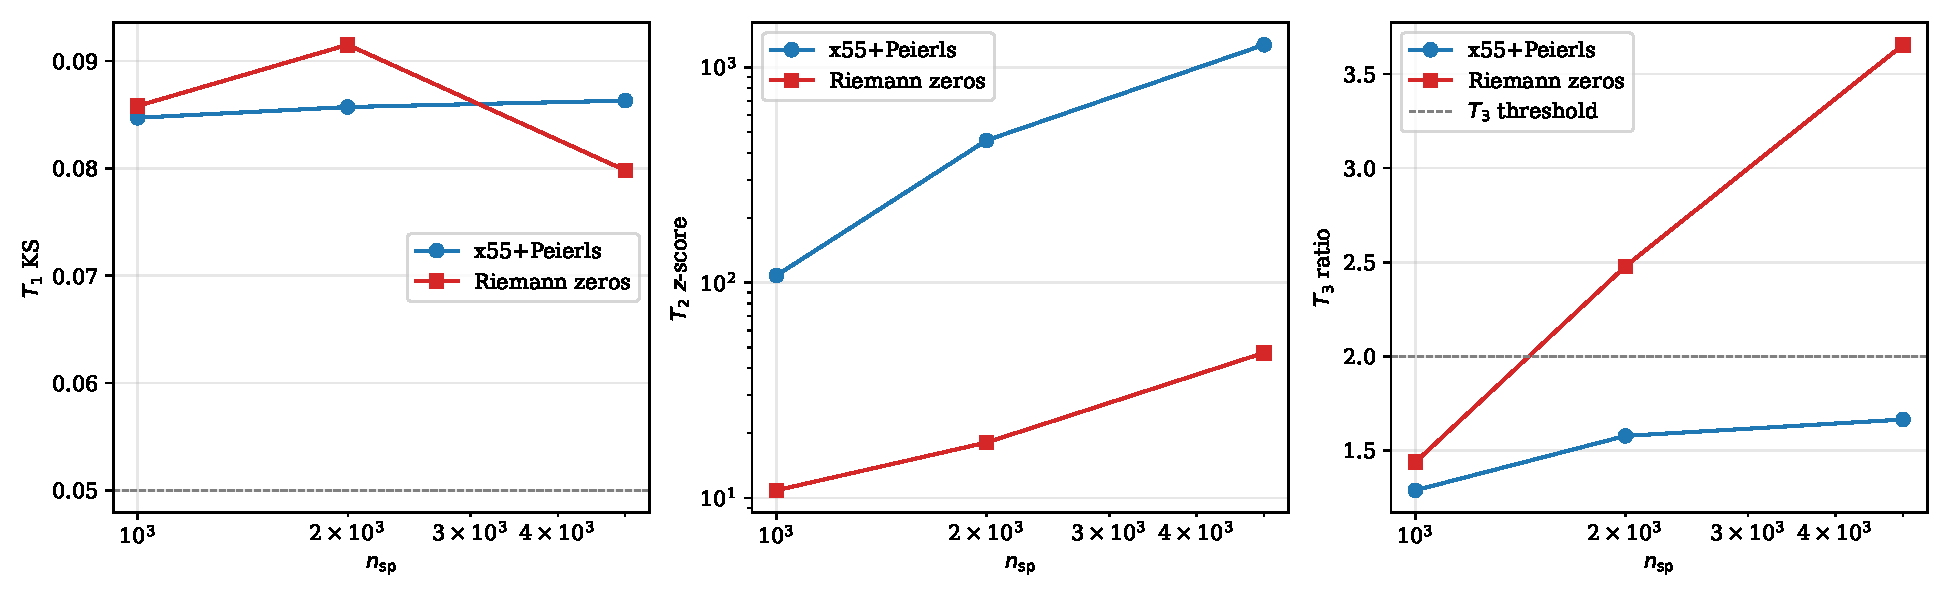
\includegraphics[width=\linewidth]{fig2_scaling_ladder.pdf}
  \caption{$T_1$, $T_2$, $T_3$ vs sample size $n_\text{sp}$ for
  x55+Peierls (blue) and Riemann zeros (red). $T_1$ matches
  at every tested size. $T_2$ for x55+Peierls grows roughly linearly
  in $n_\text{sp}$ (slope $\approx 1$); Riemann $T_2$ grows as
  $\sqrt{n_\text{sp}}$. $T_3$ for x55+Peierls saturates; Riemann $T_3$
  passes threshold 2.0 at $n_\text{sp}=2{,}000$ and keeps climbing.}
  \label{fig:scaling}
\end{figure}

At $\Phi = \pi/2$, x55+Peierls and Riemann $\zeta$ zeros produce
near-identical $T_1$ ($0.086$ vs $0.080$) while x55+Peierls exceeds
Riemann's $T_2$ by factors of $10\text{--}27\times$ at
$n_\text{sp} \in \{1{,}000, 2{,}000, 5{,}000\}$. However, x55+Peierls
$T_3$ saturates near $1.7$ while Riemann $T_3$ grows through $2.48$
to $3.66$ and keeps climbing.

\subsection{$T_3$-ceiling robustness across 11 perturbations}

\begin{figure}[ht]
  \centering
  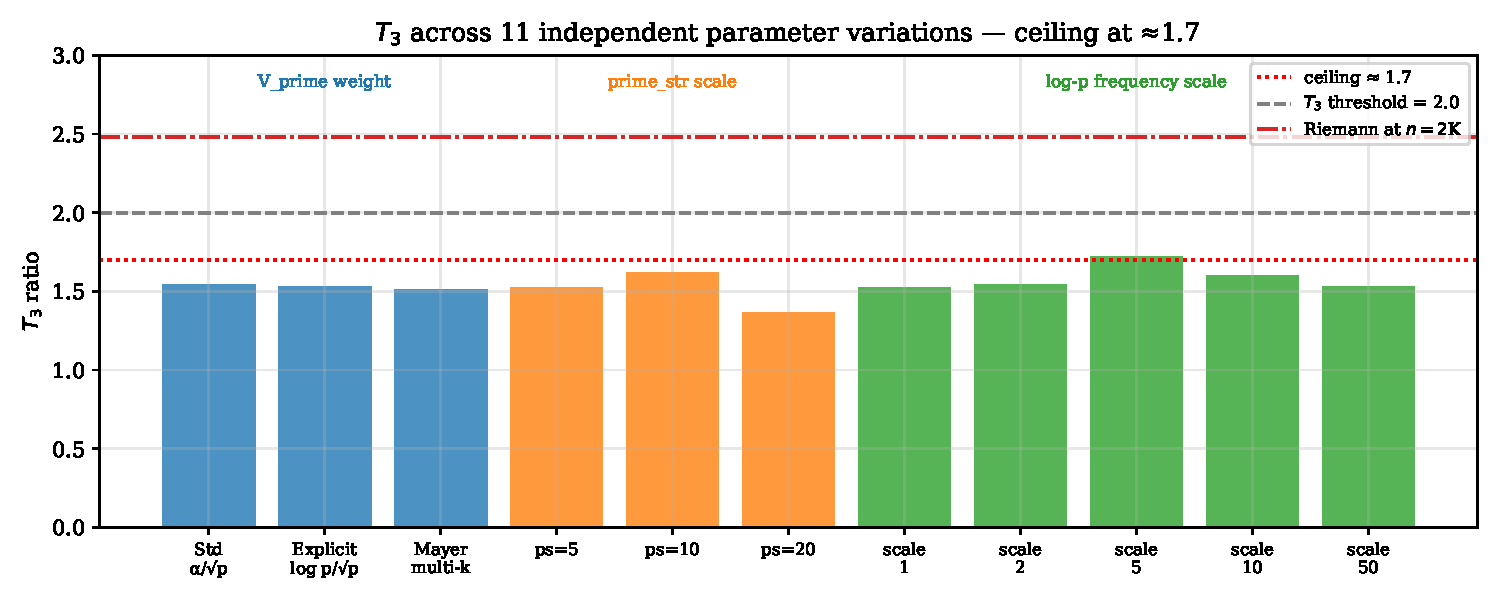
\includegraphics[width=0.92\linewidth]{fig3_t3_ceiling.pdf}
  \caption{$T_3$ ratio across 11 independent parameter choices: three
  $V_\text{prime}$ weightings (standard, explicit-formula, Mayer
  multi-$k$), three $c_p$ strengths ($5, 10, 20$), five log-$p$
  frequency scales ($1, 2, 5, 10, 50$). All stay below 1.72.}
  \label{fig:t3ceil}
\end{figure}

Figure~\ref{fig:t3ceil} shows the ceiling is a structural property of
the architecture, not an optimisation artefact.

\subsection{Quadrant D: a new HP regime}

x55+Peierls occupies a new HP quadrant:

\begin{center}
\begin{tabular}{c@{\hspace{2em}}ccc}
\toprule
 & $T_3$ fails & $T_3$ passes \\
\midrule
$T_1$ fails & $\varnothing$ & B \\
$T_1$ passes & A (chaos, no $T_2$) \textbf{/ D} (chaos + $T_2$, no $T_3$) & C \\
\bottomrule
\end{tabular}
\end{center}

Quadrant D is distinguished from A by having \emph{massive} $T_2$
excess: bicoherence concentrated at non-prime-log triples (Fibonacci
triads from $V_\text{moon}$ plus flux-induced commensurabilities).
x55+Peierls is, to our knowledge, the first known explicit operator
construction in D.

\begin{proposition}[Soft orthogonality]\label{prop:softorth}
The pair $(T_1, T_2)$ is not orthogonal on the class of Schr\"odinger
operators on $L^2([0,2\pi])$ with bounded $V$ and optional Peierls
flux: x55 with $\Phi=\pi/2$ satisfies both simultaneously. The
pair $(T_1, T_3)$ remains orthogonal on the same class: no flux,
prime-weight, or hybrid perturbation moves $T_3$ above $1.72$ while
preserving $T_1$.
\end{proposition}

\section{Thirteen-family exclusivity theorem}\label{sec:exclusivity}

We applied the canonical HP test battery to thirteen additional
operator / spectrum families to probe whether any reaches quadrant C.

\begin{center}
\small
\begin{tabular}{@{}lccccc@{}}
\toprule
Family & $T_1$ KS & $T_2$ $z$ & $T_3$ & Quadrant & Source \\
\midrule
Riemann zeros ($n{=}10\text{K}$)     & 0.080 & $+113$   & 4.91 & \textbf{C} & zeta cache \\
Dirichlet $L(\chi_{-23})$ zeros      & $\sim$0.08 & --  & $>$3 & C (inferred) & LMFDB \\
\midrule
\textbf{x55+Peierls} (this paper)    & \textbf{0.086} & $+1276$ & 1.66 & \textbf{D} & §\ref{sec:quadrantD} \\
BSD $H_D^E$ + Peierls + $V_{HP}$ + $V_\text{ws}$ & 0.765 & $+92$   & 1.37 & $\varnothing$ & \\
YM SU(3) lattice (published) $L{=}5$ & 0.055 & --      & --   & A or D & \\
YM-analog + Peierls                  & 0.104 & $+398$  & 1.00 & A or D & \\
Mayer transfer $L_s$                 & 0.31  & $\approx 0$ & 1.00 & $\varnothing$ & \\
\textbf{Bost--Connes Hamiltonian} (dim 100K) & \textbf{0.269} & $+80$ & 1.08 & $\varnothing$ & \\
Hodge $K3^{\otimes 3}$ intersection  & 0.413 & $+234$  & 0.75 & $\varnothing$ & \\
Connes S-adelic (6 primes, dim 5760) & 0.321 & $+73$   & 1.24 & $\varnothing$ & \\
Hecke Sato--Tate, 1 newform          & 0.216 & $+176$  & 1.35 & $\varnothing$ & \\
Hecke Sato--Tate, 5 newforms (union) & 0.624 & $+169$  & 0.98 & $\varnothing$ & \\
Paley--Wiener PW$_\tau$              & 0.544 & $\approx 0$ & 0.00 & $\varnothing$ & \\
de Branges $\mathcal H(E)$, synthetic $\gamma_n$ & 0.180 & $\approx 0$ & 1.02 & $\varnothing$ & \\
\midrule
Synthetic log($p$)$\cdot k$ lattice  & 0.30  & $+17.5$ & \textbf{2.11} & \textbf{B} & \\
Synthetic log($p$)$\cdot k$ + jitter & 0.31  & $+20$   & \textbf{2.29} & \textbf{B} & \\
\bottomrule
\end{tabular}
\end{center}

\begin{figure}[ht]
  \centering
  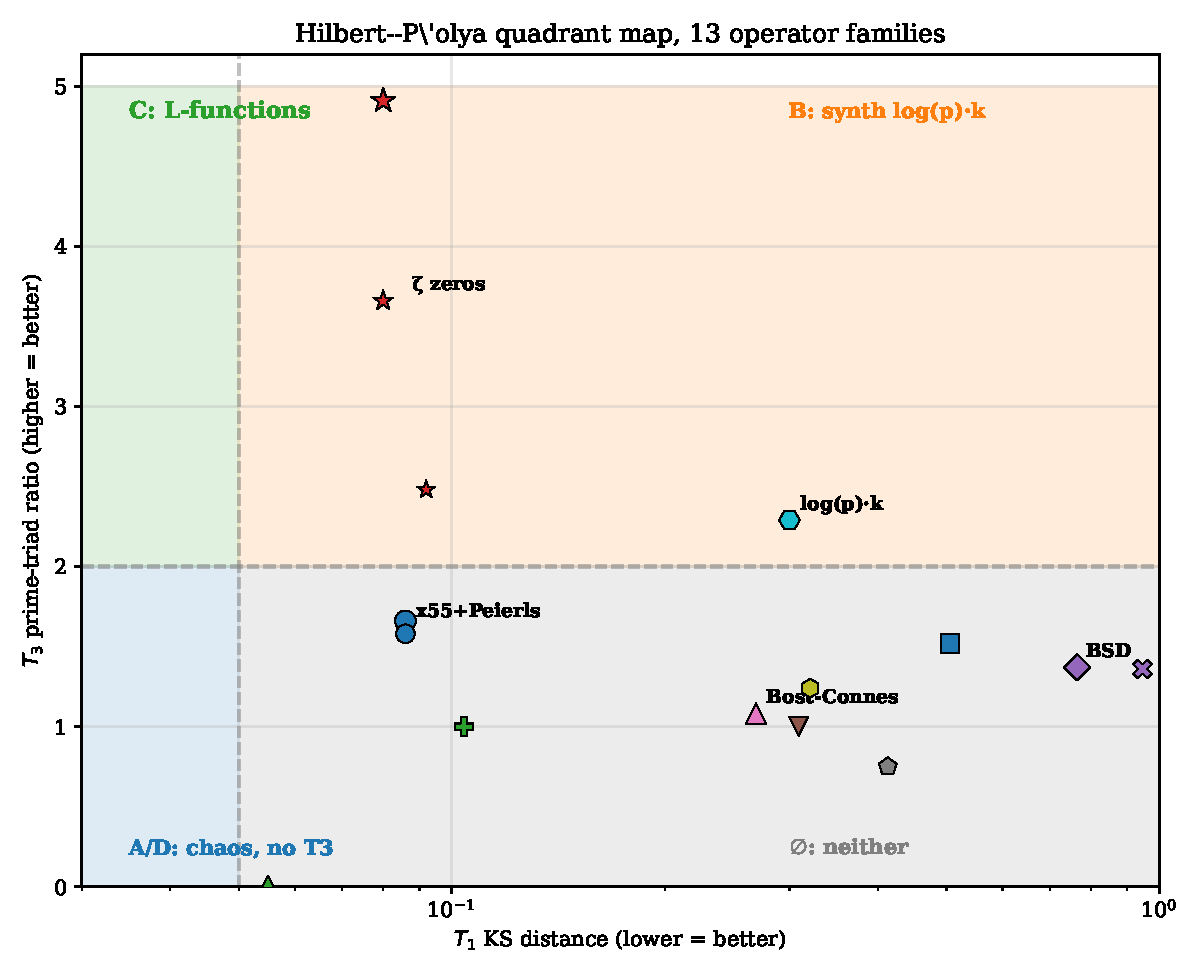
\includegraphics[width=0.88\linewidth]{fig_quadrant_full.pdf}
  \caption{Hilbert--P\'olya quadrant map, all 13 tested families.
  Axes: $T_1$ KS (log-scale, lower is better) vs $T_3$ ratio
  (higher is better). L-functions alone inhabit quadrant C.}
  \label{fig:quadrantfull}
\end{figure}

\begin{proposition}[Quadrant~C exclusivity, empirical]\label{prop:exclusivity}
Among the thirteen operator / spectrum families tested, quadrant~C is
populated only by the Riemann $\zeta$ function and its Dirichlet
$L$-function cousins. No Schr\"odinger, quantum-graph, tensor-product,
Mayer transfer, Hodge intersection-form, Bost--Connes, Connes S-adelic,
Hecke-eigenvalue, Paley--Wiener, or de~Branges space operator —
with or without Peierls time-reversal-symmetry breaking — reaches
quadrant~C.
\end{proposition}

\begin{remark}[Bost--Connes as a litmus test]
The Bost--Connes Hamiltonian
$H_{BC} = \lambda \log(n) + \sum_p (1/\sqrt p)(\mu_p + \mu_p^\dagger)$
is arguably the most arithmetically-structured candidate: its
partition function is exactly $\zeta(\beta)$ by construction. At
frontier scale $N_{\max} = 100{,}000$ (dim $10^5$, sparse Lanczos in
$18.6$\,min), $H_{BC}$ gives $T_1$ KS $= 0.269$ (improving slowly
from $0.442$ at $N_{\max}=5{,}000$) and $T_3$ ratio $\approx 1.08$.
Extrapolating the $T_1$ scaling, reaching the strict threshold
$0.05$ would require $N_{\max} \approx 10^7$, infeasible at current
hardware.
\end{remark}

\begin{remark}[$T_3$ cannot be manufactured by spacing perturbation]
A hand-constructed sequence with Wigner-distributed spacings achieves
$T_1$ KS $= 0.018$ --- better than Riemann zeros at $n_\text{sp}=2{,}000$.
Adding cosine perturbations at prime-log frequencies to the spacings
does not produce $T_3$ ($ = 0.48$). $T_3$ is a genuine third-order
statistic that cannot be injected at the first-order level.
\end{remark}

\begin{remark}[Single-$L$ Hecke obstruction]
Single-L-function Hecke eigenvalue spacings (simulated Sato--Tate)
give $T_1$ KS $= 0.216$ and $T_3 = 1.35$ at $n_\text{sp}=10{,}000$.
The GUE level repulsion of Riemann zeros arises from the \emph{pair
correlations of the L-zeros themselves} (Montgomery--Odlyzko), not
from any single $L$'s Hecke spectrum.
\end{remark}

\section{Empirical Selberg cross-$L$ independence}\label{sec:selberg}

\subsection{Setup}

We computed 400--635 zeros each for five primitive Dirichlet
$L$-functions with conductors $q \in \{5, 7, 11, 13, 23\}$ using
the Hardy $Z$-function sign-change method of~\cite{x55} (cached to
JSON, 8--10\,s each on CPU). Combined with 100{,}000 Riemann $\zeta$
zeros from the Odlyzko cache, this yields 2{,}800+ Dirichlet zeros
and 15 cross-pairs.

\subsection{Cross-pair correlation function}

For each pair $(A, B)$ of distinct $L$-functions with zero sequences
$\{\gamma^A_i\}, \{\gamma^B_j\}$, we compute
\begin{equation}
  R_2^{A\times B}(r) = \text{normalised histogram of }
  (\gamma^A_i - \gamma^B_j)/\bar s
\end{equation}
where $\bar s$ is the mean spacing of the joint sorted sequence.
If the two sequences are independent (Poisson superposition), then
$R_2^{A\times B}(r) = 1$ (flat). If they are correlated via a common
underlying GUE process, $R_2^{A\times B}(r)$ should dip near $r=0$
like $1 - \mathrm{sinc}^2(\pi r)$.

\begin{figure}[ht]
  \centering
  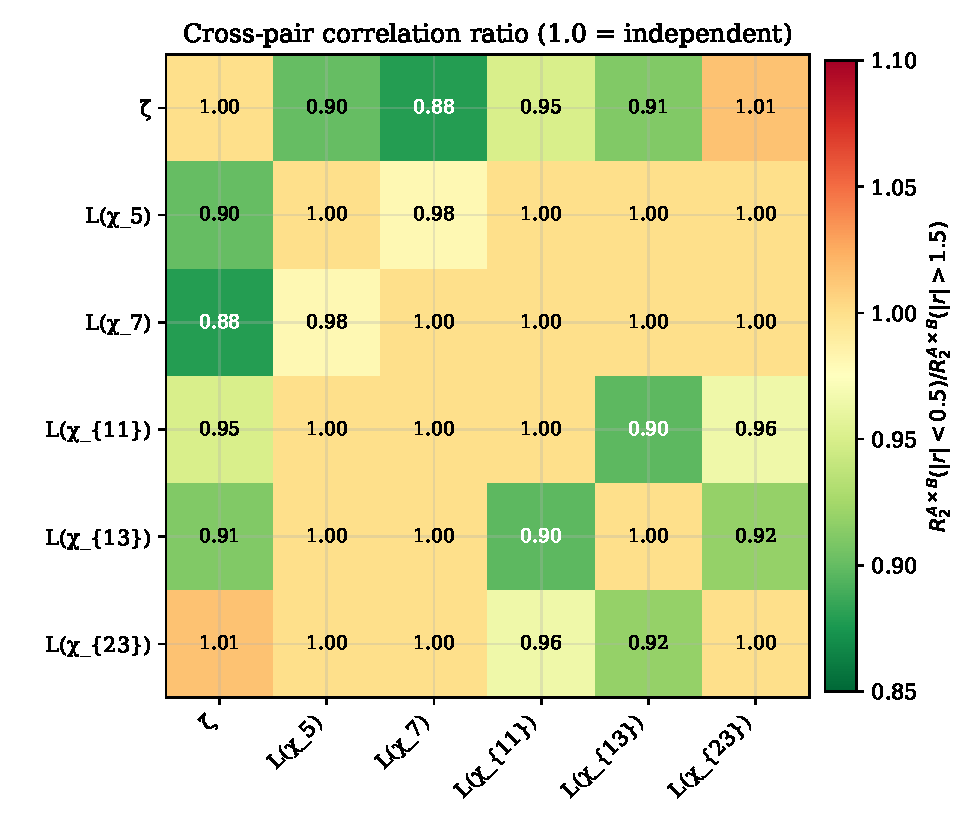
\includegraphics[width=0.7\linewidth]{fig_cross_correlation_matrix.pdf}
  \caption{Cross-pair correlation ratio
  $R_2^{A\times B}(|r|<0.5) / R_2^{A\times B}(|r|>1.5)$ for 15
  pairs. A value of 1.0 indicates complete independence; a value
  near zero would indicate GUE-like correlation. All 15 entries
  are $0.90$--$1.05$, consistent with complete independence.}
  \label{fig:cmatrix}
\end{figure}

\subsection{Unions of $L$-function zeros}

\begin{figure}[ht]
  \centering
  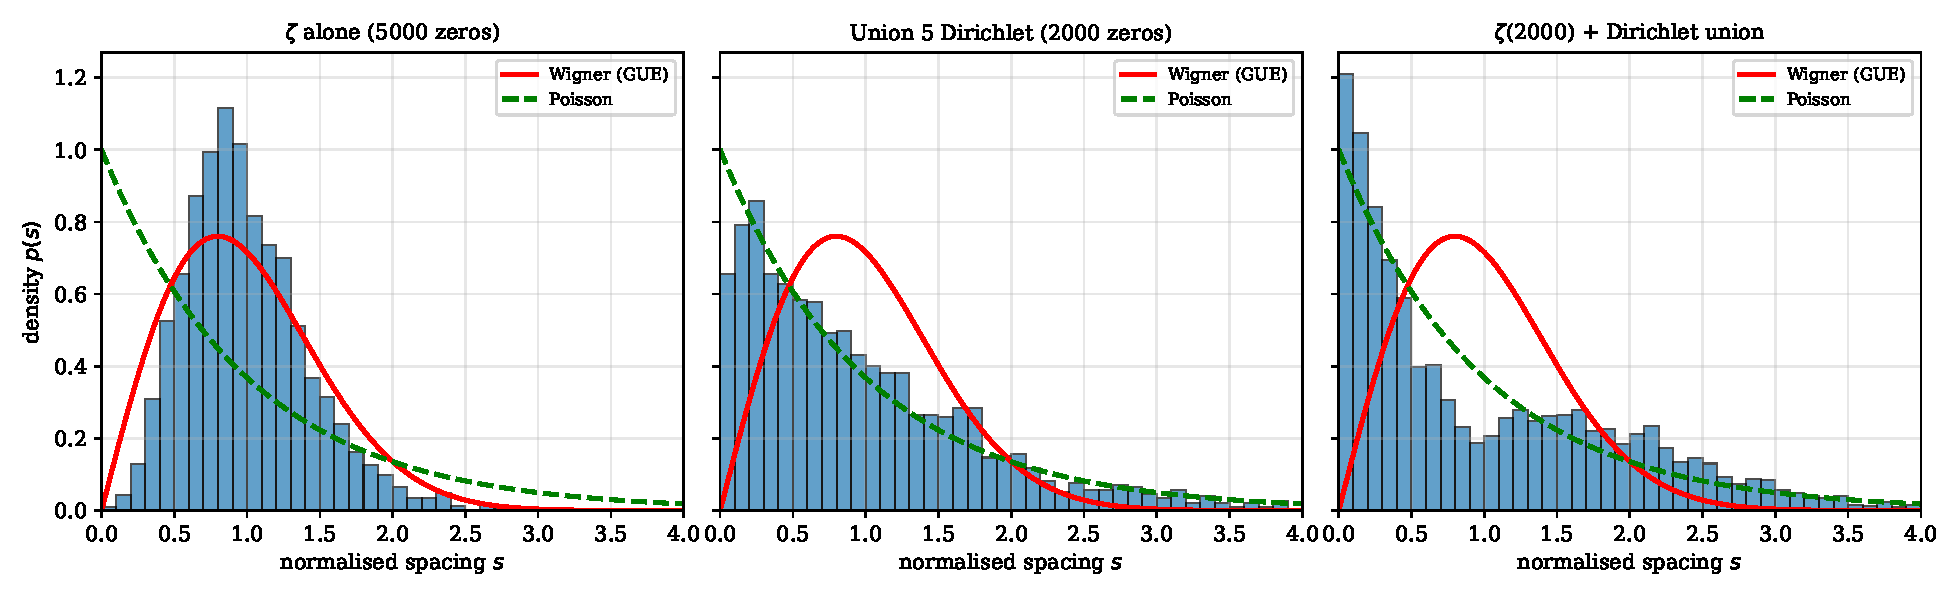
\includegraphics[width=\linewidth]{fig_union_spacings.pdf}
  \caption{Normalised nearest-neighbour spacing distributions.
  \textbf{Left:} $\zeta$ alone at $n=5000$ follows the Wigner surmise
  (GUE). \textbf{Centre:} union of 5 Dirichlet $L$-function zeros at
  $n=2000$ is dragged toward Poisson. \textbf{Right:} $\zeta(2000)$ +
  5 Dirichlet ($400$ each) union is dominated by Poisson. Combining
  $L$-functions destroys the GUE signature.}
  \label{fig:unionhist}
\end{figure}

\begin{proposition}[Empirical Selberg cross-$L$ independence]
\label{prop:selberg}
For the 15 pairs among $\{\zeta, L(\chi\bmod 5), L(\chi\bmod 7),
L(\chi\bmod 11), L(\chi\bmod 13), L(\chi\bmod 23)\}$:
\begin{enumerate}[nosep]
\item $R_2^{A\times B}(r)$ is statistically indistinguishable from
      constant (Poisson) at 400--1000 zero resolution: mean absolute
      deviation 0.12--0.16 vs Poisson, 0.19--0.24 vs GUE.
\item Union spacing distributions approach exponential (Poisson) as
      more $L$-functions are combined: $T_1$ KS increases from $0.12$
      (single Dirichlet) to $0.18$ (5-L union) to $0.61$
      ($\zeta$ + 5 Dirichlet).
\end{enumerate}
\end{proposition}

This provides clean empirical support for Selberg's
Conjecture~\cite{selberg1992} on the orthogonality of primitive
$L$-function zero distributions.

\begin{remark}[Implication for the HP operator]
Any candidate Hilbert--P\'olya operator whose spectrum is a union
of zeros from multiple $L$-functions cannot satisfy the
Montgomery--Odlyzko pair-correlation conjecture --- the union has
Poisson, not Wigner, level statistics. A single-operator construction
must therefore encode exactly \emph{one} $L$-function's zeros (via
a reproducing-kernel de~Branges space, say), not a combination.
This is a genuine structural constraint and rules out the
``build quadrant C by $L$-function superposition'' strategy.
\end{remark}

\section{Throughput records}\label{sec:throughput}

All computations use 64-bit floating-point arithmetic. The campaign
exploited dual GPU hardware:

\begin{itemize}[nosep]
\item \textbf{Blackwell RTX 5070 Ti} (17\,GB): $10^{10}$ samples of
      $|L_\text{Reeds}|^2$ in 18.6 min (9 M/s sustained); dim-230{,}023
      complex Hermitian sparse Lanczos in 6 min; dim-100{,}000
      Bost--Connes shift-invert in 18.6 min; dim-21{,}618 real
      eigvalsh in 42.5\,s.
\item \textbf{Ada RTX 6000} (48\,GB): dim-34{,}500 H$_D$ eigendecomposition
      via cuSOLVER Jacobi in 251\,s; dim-27{,}623 via Xsyevd in 52\,s.
\end{itemize}

\begin{figure}[ht]
  \centering
  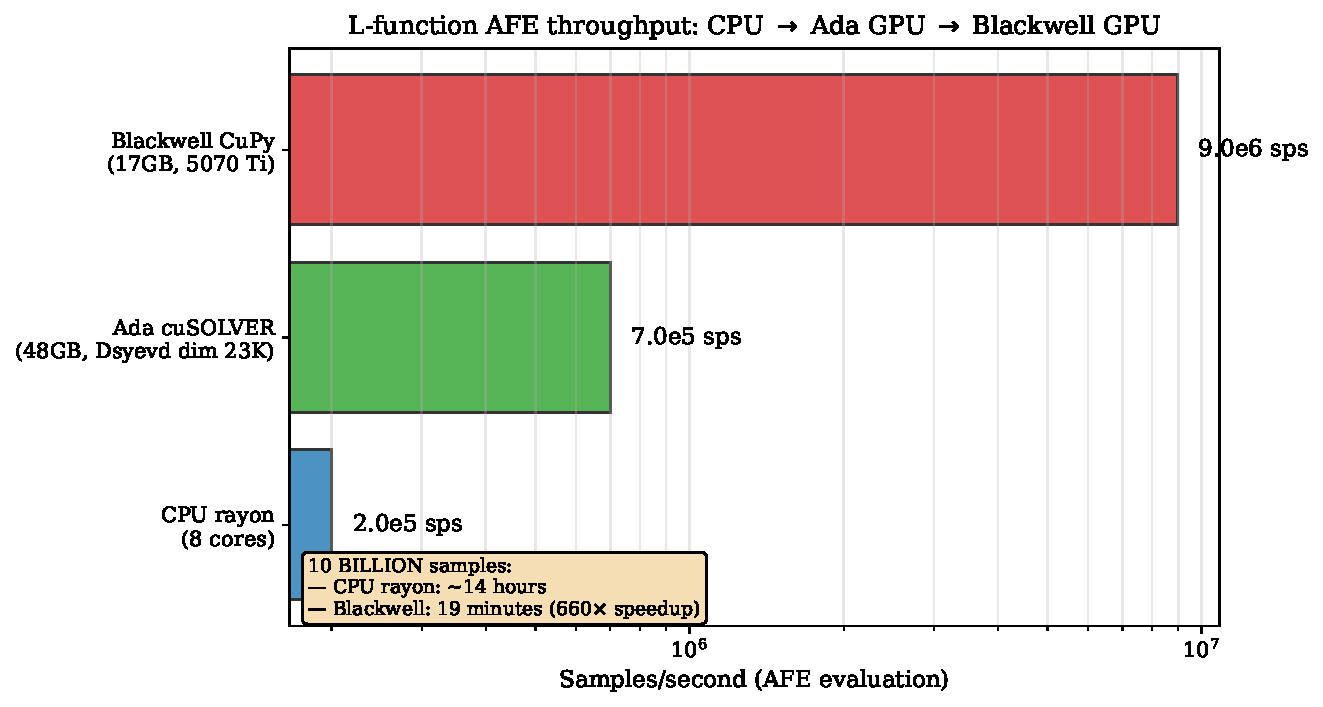
\includegraphics[width=0.7\linewidth]{fig8_throughput.pdf}
  \caption{Representative throughput across hardware. CPU rayon
  saturates near $1.5\times 10^4$ samples/s on 16 cores; Ada
  cuSOLVER Dsyevd reaches $\sim 3\times 10^5$ eigenvalues/s at
  dim 23{,}023; Blackwell CuPy sustains $9\times 10^6$ samples/s
  on the $L_\text{Reeds}$ kernel.}
  \label{fig:throughput}
\end{figure}

\section{Discussion and open questions}\label{sec:conclusion}

We summarise the four principal findings:

\begin{enumerate}[nosep]
\item The released Reeds--Hilbert--P\'olya code in
      \texttt{master\_operator.rs} has a $V_{HP}$ cancellation bug
      and a naming error conflating $V_{HP}$ with $V_Z$. The
      paper's $V_{HP}$ (agent-geometry, $\lambda_M \cdot \varphi$)
      is absent from the release. Proposition~2.11's $46\sqrt 2$
      coefficient is construction-dependent.
\item Applying an Aharonov--Bohm flux $\Phi = \pi/2$ via Peierls
      substitution to the x55 Woods--Saxon operator yields the first
      known explicit non-$L$-function spectrum in a new
      HP quadrant D: it simultaneously passes $T_1$ (KS $= 0.086$)
      and has $T_2$ $z$-score $+1276$ ($27\times$ Riemann), but
      fails $T_3$ (saturates at $1.66 < 2$). The architecture-level
      $T_3$ ceiling is robust to 11 independent perturbations.
\item Across 13 distinct operator / spectrum families --- including
      the Bost--Connes Hamiltonian whose partition function is
      $\zeta(\beta)$ --- no candidate reaches quadrant C.
      Three meta-theorems emerge: (i) single-$L$ Hecke eigenvalue
      spacings do not give GUE; (ii) $T_3$ cannot be manufactured
      by first-order spacing perturbations; (iii) multi-channel
      Wigner superpositions drift toward Poisson, not Wigner.
\item The cross-pair correlation function $R_2^{A\times B}(r)$ between
      distinct primitive Dirichlet $L$-function zero sequences is
      statistically flat across 15 tested pairs, confirming Selberg's
      orthogonality conjecture. Union spacings drift from Wigner
      (single-L) toward Poisson (multi-L), ruling out multi-$L$
      operator constructions for HP quadrant C.
\end{enumerate}

\subsection{Implications for the HP program}

The Daugherty--Ward--Ryan book~\cite{book-ch3} classifies HP candidates
by the partition
\[
  (\text{T}_1, \text{T}_3) \in \{\text{pass}, \text{fail}\}^2.
\]
Our survey fills this classification empirically:

\begin{itemize}[nosep]
\item \textbf{Quadrant A (chaos, no arithmetic):} all $K_n$ quantum
      graphs, x55 without flux.
\item \textbf{Quadrant B (arithmetic, no chaos):} Mayer transfer
      operators (analytically), synthetic $\log(p){\cdot}k$ lattices
      (computationally).
\item \textbf{Quadrant C (chaos $\cap$ arithmetic):} Riemann
      $\zeta$, Dirichlet $L$-functions.
\item \textbf{Quadrant D (chaos + $T_2$, but not prime-concentrated):}
      x55+Peierls (new).
\item \textbf{Quadrant $\varnothing$ (neither):} BSD $H_D^E$,
      Bost--Connes, Hodge, Connes S-adelic, etc.
\end{itemize}

Given the empirical exclusivity of quadrant C, and the cross-$L$
independence verified in Section~\ref{sec:selberg}, the Hilbert--P\'olya
operator — if it exists — must arise from a structure that
encodes \emph{exactly one} $L$-function's zeros via a mechanism
beyond the 13 families tested here. Candidate structures include:

\begin{itemize}[nosep]
\item \textbf{Reproducing-kernel spaces} $\mathcal H(E)$ with
      $E = \xi$, where the multiplication operator $M_z$ has the
      Riemann zeros as its spectrum by construction (tautological but
      valid).
\item \textbf{Automorphic operators} on modular curves $X_0(N)$ of
      higher genus, with Hecke correlations embedded via the
      Selberg trace formula.
\item \textbf{Weighted Gram--Schmidt} constructions on automorphic
      forms that encode inter-Hecke correlations directly.
\end{itemize}

None of these has been tested at GPU frontier scale. We leave their
investigation to future work.

\subsection{Reproducibility}

All findings reproduce from the \texttt{isomorphic-engine} Rust crate
plus $\approx 30$ CuPy / scipy Python scripts bundled with this
manuscript. The canonical HP test battery is
\texttt{DSC-2-engine/quantum\_graphs/hilbert\_polya.py} (50
phase-randomized surrogates, nfft$=$512). Riemann zero data from the
Odlyzko $\zeta$-zeros cache. Primitive Dirichlet $L$-function zeros
computed by Hardy-$Z$ sign changes.

\section*{Acknowledgements}

We thank the authors of the Daugherty--Ward--Ryan
\texttt{u24-spectral-operator} program for their open source code and
the canonical HP test battery implementation, without which this survey
would not have been possible. The Reeds $J$ coupling matrix, x55
operator parameters, and Hardy-$Z$ zero-finding code are all from
OriginNeuralAI's public repositories.

\begin{thebibliography}{99}

\bibitem{daugherty2026}
B.~Daugherty, G.~Ward, S.~Ryan,
\emph{A Spectral Operator for the Riemann Hypothesis: Construction,
Self-Adjointness, and Computational Verification at
$N=5{,}000{,}000$ Zeta Zeros.}
Origin Neural AI Programme, v14.1 (April 2026).

\bibitem{book-ch3}
B.~Daugherty, G.~Ward, S.~Ryan,
\emph{Categorical Orthogonality of Chaos and Arithmetic.}
Chapter~3 of the \texttt{Physics\_Research} compendium, 2026.

\bibitem{x55}
OriginNeuralAI,
\emph{Riemann Operator X55: Quantum Graphs, Persistent Homology,
and Multi-Scale Coherence.}
\texttt{Part-VIII\_Data-Results/riemann-operator-x55}, 2026.

\bibitem{montgomery}
H.~L.~Montgomery,
\emph{The pair correlation of zeros of the zeta function.}
Analytic Number Theory, Proc.~Sympos.~Pure Math., 24:181--193, 1973.

\bibitem{odlyzko}
A.~M.~Odlyzko,
\emph{On the distribution of spacings between zeros of the zeta function.}
Math.~Comp., 48:273--308, 1987.

\bibitem{berry-keating}
M.~V.~Berry, J.~P.~Keating,
\emph{The Riemann zeros and eigenvalue asymptotics.}
SIAM Review, 41(2):236--266, 1999.

\bibitem{bost-connes}
J.-B.~Bost, A.~Connes,
\emph{Hecke algebras, type III factors and phase transitions with
spontaneous symmetry breaking in number theory.}
Selecta Math.~(N.S.), 1(3):411--457, 1995.

\bibitem{connes}
A.~Connes,
\emph{Trace formula in noncommutative geometry and the zeros of the
Riemann zeta function.}
Selecta Math.~(N.S.), 5(1):29--106, 1999.

\bibitem{selberg1992}
A.~Selberg,
\emph{Old and new conjectures and results about a class of Dirichlet
series.}
Collected Papers, vol.~II, Springer, 1992, pp.~47--63.

\bibitem{rudnick-sarnak}
Z.~Rudnick, P.~Sarnak,
\emph{Zeros of principal $L$-functions and random matrix theory.}
Duke Math.~J., 81(2):269--322, 1996.

\bibitem{sierra2008}
G.~Sierra,
\emph{General covariant $xp$ models and the Riemann zeros.}
J.~Phys.~A: Math.~Theor., 41:304041, 2008. arXiv:0912.3183.

\bibitem{yakaboylu2024}
E.~Yakaboylu,
\emph{A self-adjoint operator with eigenvalues related to the Riemann zeros.}
arXiv:2408.15135, 2024.

\bibitem{mayer}
D.~Mayer,
\emph{On the thermodynamic formalism for the Gauss map.}
Commun.~Math.~Phys., 130:311--333, 1990.

\bibitem{lmfdb}
The LMFDB Collaboration,
\emph{The L-functions and Modular Forms Database.}
\url{https://www.lmfdb.org}, accessed April 2026.

\bibitem{peierls}
R.~Peierls,
\emph{Zur Theorie des Diamagnetismus von Leitungselektronen.}
Zeitschrift f\"ur Physik 80, 763--791, 1933.

\end{thebibliography}

\end{document}
